%% The following is a directive for TeXShop to indicate the main file
%!TEX root = ../MJThesis.tex
\acresetall
\chapter{OmpW of \textit{Caulobacter crescentus} functions as an outer membrane channel}
\label{ch:porin}
\begin{epigraph}
  \emph{``We must never let ourselves fall in thinking `ignorabimus' (`We shall never know'), but must have every confidence that the day will dawn when even those processes of life which are still a puzzle today will cease to be inaccessible to us natural scientists.''} ---~Eduard~Buchner,~1907~Nobel~lecture 
\end{epigraph}
\section{Introduction} % (fold)
\label{sec:porin_introduction} 
\lettrine[lines=2]{G}{ram-negative} bacterial cell-envelopes consist of different layers. The inner, or cytoplasmic, membrane contains the respiration chain, proteins for the transport of nutrients, and proteins involved in the synthesis of phospholipids, peptidoglycan, and lipopolysaccharides\upcite[.]{beveridge1981ultrastructure, nikaido1985molecular} The periplasmic space between the membranes is an aqueous compartment isoosmolar to the cytoplasm\upcite[.]{benz1994uptake} It contains the peptidoglycan and a large number of different proteins. The outer membrane is composed of protein, lipid and \ac{LPS}\upcite[.]{beveridge1981ultrastructure} It typically contains only a few major proteins. Normally at least one of the constitutive outer membrane proteins is a porin, a general diffusion pore with a defined exclusion limit for hydrophilic solutes\upcite[.]{nikaido2003molecular} In addition to constitutive porins, an outer membrane may contain porins that are induced under special growth conditions\upcite[.]{benz2001porins} They often form solute-specific channels and contain binding sites for neutral substrates such as carbohydrates\upcite[,]{benz1986pore, ferenci1980lambda} or nucleosides\upcite[,]{benz1986pore} and phosphate\upcite[.]{benzhancock1987mechanism, hancock1982outer} Many of the specific porins are part of uptake and degradation systems, such as the maltose uptake system of \ac{ecoli}\upcite[.]{schwartz1987maltose} 
% Add more intro to porins? 

    \ac{caulobacter}, an alphaproteobacterium found in oligotrophic aquatic environments\upcite[.]{curtis2010getting}, is an unusual Gram-negative bacterium in that genes coding for typical general diffusion porins of the OmpF/C type of enteric Gram-negative bacteria have not been identified in its genome\upcite[.]{lohmiller2008tonb, neugebauer2005exbbd, caulobactergenomeseq} Similarly, genes coding for specific porins such as Tsx or LamB are also absent. To date, no definitive porin has been demonstrated in \caulobacter. Instead, the genome of \ac{caulobacter} contains a large number of genes that code for TonB-dependent receptors\upcite[.]{lohmiller2008tonb, neugebauer2005exbbd} More than 60 of these receptors have been identified\upcite[,]{lohmiller2008tonb} which probably means that most of the nutrients from dilute environments are taken up actively by these systems. Examples for this are the uptake of maltose and \ac{glcnac} into the cells\upcite[,]{eisenbeis2008naga, lohmiller2008tonb}, as opposed to the passive mechanisms of porins.

    In this study we investigated whether the outer membrane of \ac{caulobacter} also contained a porin-like channel. The results suggest that  a porin-like channel could be detected in artificial membranes with a single-channel conductance of about 125 \si{\pico\sievert} in 1 \si{\molar} \ce{KCl}. The protein responsible for channel formation has been identified to be a member of the large OmpW family of outer membrane proteins. OmpW analogue proteins are found in many Gram-negative bacteria. Two members of this family, OmpW of \ac{ecoli} and OprG of \ac{pseudomonas} have been crystallized and their 3D-structures are known at high resolution (2.7 and 2.4 \AA, respectively)\upcite[.]{albrecht2006expression, hong2006outer, touw2010crystal}  OmpW of \ac{caulobacter} functions as a channel for cations, which is in sharp contrast to OprG of \ac{pseudomonas} and OmpW of \ecoli, which are believed to be plugged completely or involved in the transport of small, yet unknown hydrophobic molecules across the cell wall of these bacteria\upcite[.]{albrecht2006expression, hong2006outer, touw2010crystal} The 3D-structure of OmpW of \ac{caulobacter} was modeled on the basis of the known structures of OmpW of \ac{ecoli} and OprG of \ac{pseudomonas}\upcite[.]{hong2006outer, touw2010crystal} The results indicated that OmpW of \ac{caulobacter} could have a larger diameter and more hydrophilic interior than the two crystallized members of the OmpW family.

\section{Methods and Materials}
\label{sec:porin_methods}
\subsection{Growth and maintenance of microorganisms} 
\label{sub:porin_growth}
\caulobacter NA1000 353$\Phi$ (JS1013), a strain that carries an amber mutation in the gene rsaA resulting in S-layer deficiency\upcite[,]{ford2007s} was used for initial identification and characterization of OmpW. Wildtype \caulobacter NA1000 was used for generating an ompW-knockout strain and as a comparison against the knockout strain. The bacteria were  grown to mid log phase (\ac{OD600} $\approx$ 0.8) in \ac{PYE}\upcite{poindexter1964biological} at 30\si{\degreeCelsius} in 5 \millilitre cultures, which were used to start large cultures in 2.8 \si{\litre} Fernbach flasks containing 1250 \millilitre M16HIGGG medium, shaken at 100 rpm. M16HIGG is a modification of M6HIGG medium\upcite[,]{smit1981periodic} containing 0.31\% glucose, 0.09\% glutamate, 1.25 mM sodium phosphate, 3.1 mM imidazole, 0.05\% ammonium chloride and 0.5\% modified Hutner’s Mineral Base.

\subsection{Outer membrane enriched preparations}
\label{sub:porin_omp_prep}
The protocol for preparing outer membrane extracts enriched in OmpW was derived from our \ac{LPS} isolation protocol (on \cpageref{sub:LPS_isolation}). The really crucial difference here, is the omission of proteinase K. The lack of a nuclease step was primarily for conveinence, but also it was deemed unessecary. Nucleic acids can be significant contaminants in \ac{NMR} analysis, even in trace quantities, but they are not a serious concern in the these bilayer  experiments or \ac{SDS-PAGE} analyses.

Cells were pelleted by centrifugation at 12,400 x g for 10 min. Cell pellets were washed by suspension with distilled water and repelleted. The pellets were resuspended in 1/10 original culture volume of \ac{PBS}\upcite[]{maniatis} amended with 10 \millimolar{} \ac{EDTA}, agitated at room temperature for 5 min and then centrifuged at 15,300 x g for 15 min. The supernatant was retrieved and re-centrifuged to clarify. The supernatant was then ultracentrifuged at 184,000 x g for 2 h. Glassy pellets formed which were suspended in 1/100 original culture volume in 10 \millimolar Tris pH 8.0. This treatment led preferentially to the disruption of the outer membrane and periplasmic contents were released without significantly releasing cytoplasmic contents.

\subsection{Crude membrane preparations}
    \label{sub:porin_crude_preps}
    For comparison to the \ac{PBS}-\ac{EDTA} membrane enrichment method, crude membrane preparations were prepared from 5 \millilitre of mid logarithmic culture. The culture was sonicated at 50\% intensity for 5 x 30 sec bursts. DNAse and RNAse were added to final concentrations of 0.06 \mgperml and 0.60 \mgperml respectively, and incubated at 37\si{\degreeCelsius} for 1 h. The preparation was then ultracentrifuged for 2 h at 107 000 x g. A glassy pellet formed which was resuspended in 200 \microlitre of distilled water.

\subsection{\ac{SDS-PAGE}} \label{sec:porin-sds-page}
Electrophoretic analyses of protein samples were done by the standard methods of discountinuous \ac{SDS-PAGE}\upcite[,]{laemmli} in a similar fashion to the methods used to analyze \ac{LPS} in \cref{ch:lps} on \cpageref{sub:gel_electrophoresis}. Initially, samples were boiled in sample buffer for 5 minutes prior to running on the gel. When we wanted to probe our samples for heat-modifiablitiy, samples were not boiled; to melt the sample buffer, it was heated to 37\cel prior to mixing with the protein samples. Gels were stained to visualize protein with Coomassie brilliant blue as previously described\upcite[.]{bennett1971quantitative}

\subsection{Isolation and purification of the channel-forming protein from enriched outer membranes}
\label{sub:porin_isolation}
The enriched outer membranes prepared by \ac{PBS}-\ac{EDTA} extraction was inspected for channel-forming activity by treatment with the detergent \ac{LDAO}. The detergent extracts of the enriched OM showed rapid channel formation in the lipid bilayer assay. The protein responsible for channel formation was identified by preparative \ac{SDS-PAGE}. Highest channel-forming activity was observed in the molecular mass range between 20 and 25 kDa.

Analytical and preparative \ac{SDS-PAGE} was performed according to Laemmli\upcite[.]{laemmli} The gels were stained with Coomassie brilliant blue or Colloidal Coomassie blue\upcite[.]{candiano2004blue} 

\subsection{Tryptic digestion and peptide sequencing}
\label{sub:porin_tryptic}
The pure 22 kDa protein eluted from preparative \ac{SDS-PAGE} was subjected to amino acid sequence analysis. Direct sequencing was not possible presumably because of blocking of the N-terminus. The 22 kDa protein was then cleaved with trypsin as described\upcite[.]{eckerskorn1989internal} The peptides were separated by reversed phase HPLC on a Purospher RP18 encapped 5 \si{\micro\metre} column (Merck, Darmstadt, Germany) using a solvent gradient from 0 to 60\% acetonitrile in 0.1\% trifluoroacetic acid/water (v/v). The flow rate was 60 \si{\micro\litre\per\minute} and UV-detection was performed at 206 \si{\nano\metre}. The amino acid sequence analysis of the tryptic peptides was performed using an ABI 472A protein sequencer (Applied Biosystems, Langen, Germany).

\subsection{Lipid bilayer experiments}
\label{sub:porin_bilayer}
The method used for the reconstitution experiments using black lipid bilayer membranes has been described previously\upcite[.]{benz1978formation} The membranes were formed from a 1\% (w/v) solution of diphytanoyl-\ac{PC} (Avanti Polar Lipids, Alabaster, AL, U.S.A.) in n-decane. The membrane current was measured with a pair of calomel electrodes switched in series with a voltage source and an electrometer (Keithley 617). For single-channel recordings the electrometer was replaced by a highly sensitive current amplifier (Keithley 427). Zero-current membrane potentials were measured by establishing a salt gradient across membranes containing 100--1000 channels, as has been described earlier\upcite[]{benz1979ionic, benz1985ion} using a high impedance electrometer (Keithley 617).

\subsection{Modeling of the OmpW structure}
\label{sub:porin_modeling}
The possible 3D-structure of OmpW of \ac{caulobacter} was derived using the homology modeling approach. Three dimensional model of \ac{caulobacter} OmpW was built using \texttt{Modeller} program\upcite[]{eswar2008protein} taking \ac{ecoli} OmpW as a template structure\upcite[.]{hong2006outer}
 
\subsection{Generation of \caulobacter \del ompW}
\label{sub:porin_knockout}
The gene ompW, CCNA\_01475 (CC\_1409), which encodes for OmpW, was knocked out in wildtype \caulobacter NA1000 via a two step method, derived from previously published protocols\upcite{ford2007s}, resulting in an dysfunctional copy of ompW with a large internal deletion. The amino acid sequence for OmpW can be found in the appendix on \cpageref{app:ompwseq}.

The suicide plasmid `pKMOBsacB-ompW-A/B' was constructed by combining two fragments of DNA homologous to the 5' and 3' ends of the gene ompW into a suicide vector containing both positive and negative selection elements. The `A-fragment' was \ac{PCR} amplified using the primers F-ompW-A (5'- \texttt{TAC CGG AAT TCT CGG GCG CTG GGC CTG TCT GTT GAG }-3') and R-ompW-A (5'-\texttt{ GTC CCA AGC TTG CGG AAG ATC TAT TGG CGC CGG CGG CAG TCA GGA TG }-3'), resulting in a 994 bp product with a 5' \textit{Eco}RI cleavage site and  3' \textit{Bgl}I and \textit{Hin}DIII cleavage sites.  The `A-fragment' \ac{PCR} product was blunt ligated in to pBSK-ESH\upcite[,]{rsaf} resulting in pBSK-ompW-A. The `B-fragment' PCR product was amplified using the primers F-ompW-B (5'- \texttt{CGG GAT CCA CGT CAA GAA GGT CTA TTT CAG CAC }-3' and R-ompW-B (5'- \texttt{GTC CCA AGC TTG CGT CGA TGC TAG TGC GCT GCG ATG }-3'), resulting in a 1090 bp product with a 5' \textit{Bam}HI cleavage site and a 3' \textit{Hin}DIII cleavage site. The `B-fragment' \ac{PCR} product was similarly blunt subcloned into pBSK-ESH, then excised by \textit{Bam}HI and \textit{Hin}DIII digestion, and ligated into pBSK-ompW-A, digested with \textit{Bgl}II and \textit{Hin}DIII, resulting in the plasmid pBSK-ompW-A/B. The plasmids pBSK-ompW-A/B and pKMOBsacB were digested with \textit{Eco}RI and \textit{Hin}DIII, the 2070 bp fragment from pBSK-ompW-A/B was ligated into the pKMOBsacB fragment creating the plasmid pKMOBsacB-ompW-A/B.

The plasmid pKMOBsacB-ompW-A/B was electroporated into \caulobacter NA1000 cells\upcite[.]{gilchrist1991transformation} The resulting transformants that were kanamycin resistant were re-passaged through kanamycin-free \ac{PYE} medium three times and plated on kanamycin-free \ac{PYE} agar plates that contain 3\% sucrose. All colonies that were found to be sucrose resistant were screened for kanamycin sensitivity to confirm that the pKMOBsacB-ompW-A/B plasmid had crossed out of the genome. Colonies that were both sucrose resistant and kanamycin sensitive had their ompW genes \ac{PCR} amplified using the primers F-ompW (5'- \texttt{CGC ACT GGG CTT GCT GGC CTT TTT C }-3') and R-ompW (5'- \texttt{GGA GCC AGA GGA CGG ACG ACC GGG G }-3'); intact ompW resulted in a roughly 800 bp product, and knocked-out ompW resulted in a roughly 500 bp product.

% --------------------------------------------RESULTS
\section{Results}

\subsection{Protein composition of the enriched outer membranes of \textit{C. crescentus}}
Crude membranes from \caulobacter CB15A NA1000 353$\Phi$ cells that were disrupted by sonication and membrane material released by \ac{PBS}-\ac{EDTA} treatment were analyzed by \ac{SDS-PAGE}. The membranes from the sonicated cells (presumably a mixture of the cytoplasmic and outer membranes) (\cref{fig:porin-pbsedtagel}, lane 1) and the membranes from the \ac{PBS}-\ac{EDTA} extract (\cref{fig:porin-pbsedtagel}, lane 2) showed numerous proteins present, whereas the \ac{PBS}-\ac{EDTA} extracted cell membranes (not boiled before analysis) showed an enrichment of two protein bands at about 20 and 22 kDa. When the \ac{PBS}-\ac{EDTA} extract preparations were boiled prior to \ac{SDS-PAGE}, the two enriched bands resolved as a single band of about 22 kDa in size (\cref{fig:porin-pbsedtagel}, lane 3). This `heat modifiability' of the enriched protein (\ie lower mobility when boiled in the presence of \textsc{SDS}) is occasionally observed for Gram-negative bacterial outer membrane proteins and is probably caused by their unfolding\upcite[.]{sugawara1996secondary}

\begin{figure}[htb]
  	\begin{center}
   		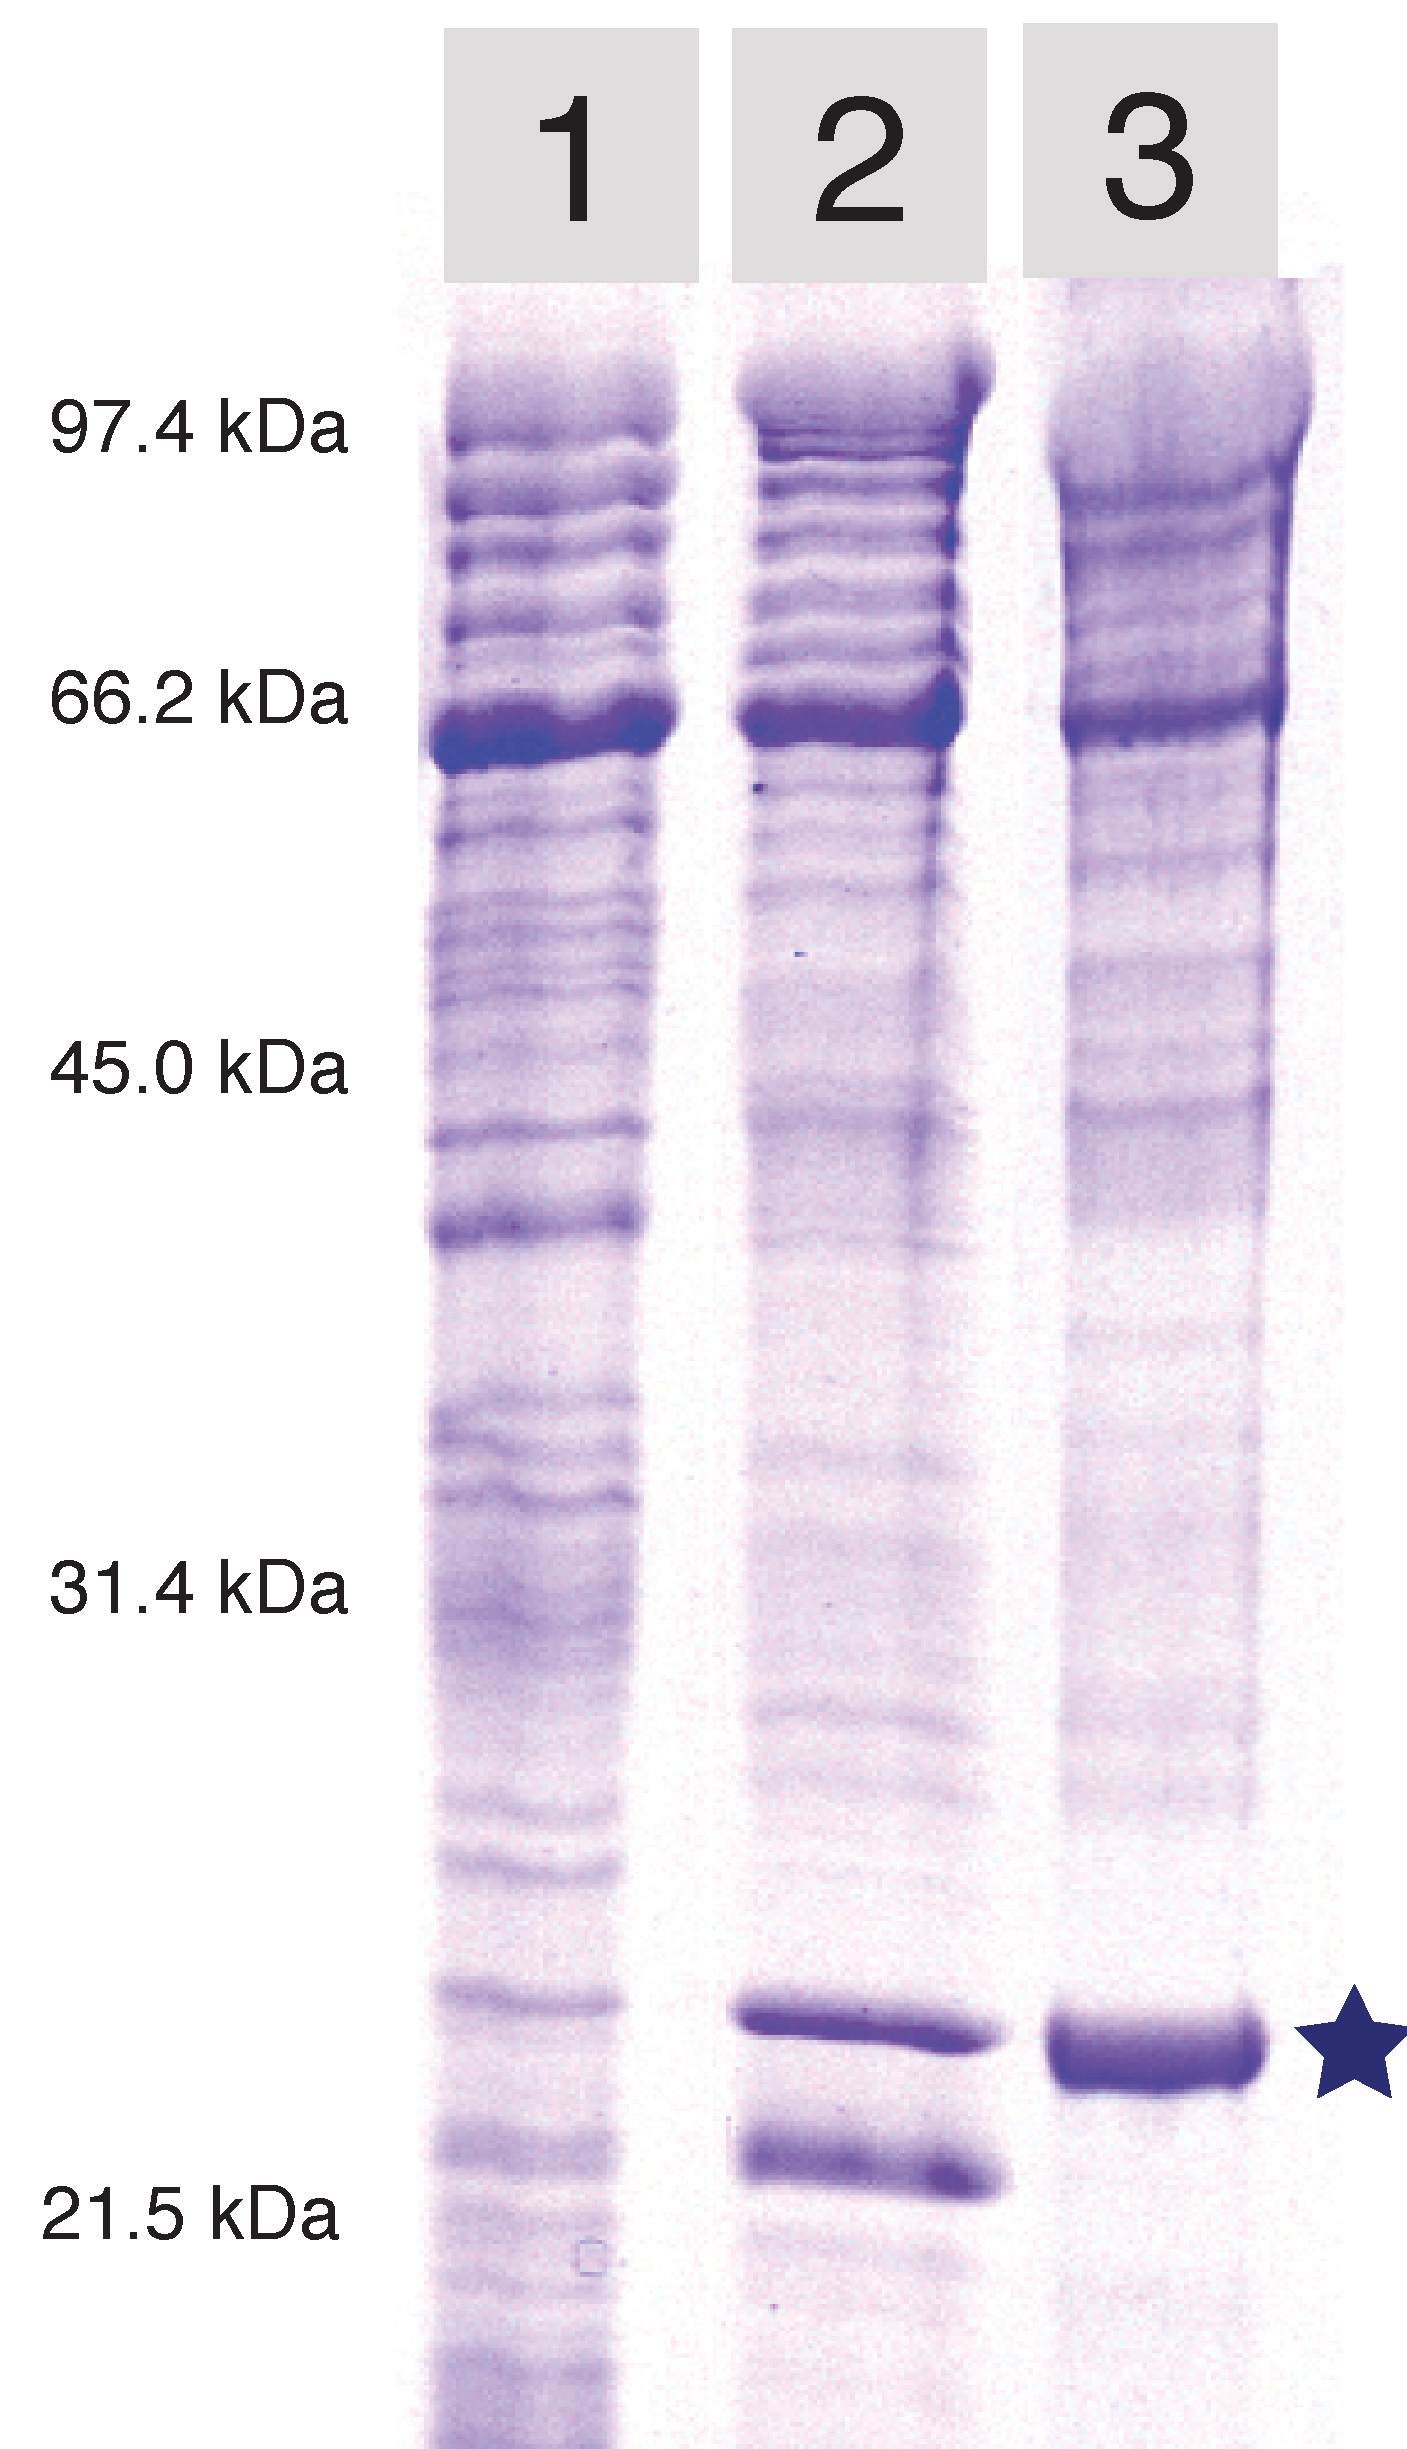
\includegraphics[width=0.2\textwidth]{porin_chapter/img/Fig1-pbsedta.pdf}
   	\end{center}
   	\caption[Coomassie stained \ac{SDS-PAGE} of different protein preparations of \caulobacter.]{
	   	Coomassie stained \ac{SDS-PAGE} of different protein preparations of \caulobacter. 
Lane 1, 7.5 \microlitre of crude membrane preparation. Lane 2, 15 \microlitre of \ac{PBS}-\ac{EDTA} extract, not boiled prior to loading. Lane 3, 15 \microlitre of \ac{PBS}-\ac{EDTA} extract, boiled prior to loading. The star highlights the position of OmpW.
 	}
   	\label{fig:porin-pbsedtagel}
\end{figure}   

\subsection{Identification of channel-forming activity in enriched outer membranes of \textit{C. crescentus}}
The enriched outer membranes were treated with 0.5\% \ac{LDAO}. When small amounts of this detergent solution were added to one or both sides of a black \ac{PC}/n-decane membrane we observed a remarkable increase of membrane conductance indicating that the enriched outer membranes contained membrane-active components. %%The conductance increase was not sudden, but delayed after addition of the extract. 
After an initial rapid increase of conductance for 5--10 min, the increase slowed down and saturated at 30--60 min after addition of the detergent solution to the black membranes. Keep in mind, that when the detergent alone was added in the same concentration as with the \ac{PBS}-\ac{EDTA} extracted membranes; it had no influence on the conductance of the lipid bilayer membranes. When the detergent extract of the outer membranes was added at much lower concentrations to the aqueous phase bathing the black lipid membrane, the current increased in a step-wise fashion (see \cref{fig:porin-elutedband}A, upper panel). A histogram of the channel distribution demonstrated that most of the conductance steps had a conductance of about 125 \si{\pico\sievert} in 1M \ce{KCl} (see \cref{fig:porin-elutedband}A, lower panel). Besides the 125 \si{\pico\sievert} channel, some fluctuations with higher conductance (250 and 350 \si{\pico\sievert}) were also obtained which probably represented oligomers of the 125 \si{\pico\sievert} channel that could not be separated at the time scale of our experimental conditions. It is significant that the conductance of these steps was notably much lower than that of general-diffusion pores from enteric bacteria, which is at least 10 times higher at the same conditions (1--4 \si{\nano\sievert} in 1 M \ce{KCl}\upcite[]{benz1994uptake}). This result suggested that the \ac{PBS}-\ac{EDTA} extracted membranes of \caulobacter contained a porin-like channel of small conductance. 

\subsection{Identification of the channel-forming protein from the enriched outer membranes} 
To identify the protein responsible for the channel-forming activity, the \ac{PBS}-\ac{EDTA} extracted membranes were dissolved in detergent and subjected to preparative \ac{SDS-PAGE}. The gel was cut into thin slices, corresponding to defined molecular mass ranges, and each was eluted overnight with a buffer containing 1\% Genapol. The eluted molecular mass fractions were examined for channel-forming activity in the lipid bilayer assay. Extremely high channel-forming activity was exclusively localized within the molecular mass range around 20 to 22 kDa, corresponding to the protein bands enriched by \ac{PBS}-\ac{EDTA} extraction (see \cref{fig:porin-pbsedtagel}). The other bands from the gel, in particular the 66 kDa band, had no activity in the lipid bilayer assay. When excised and eluted, the band was again subjected to \ac{SDS-PAGE}. Without heating, the gel showed a single protein band of about 20 kDa suggesting that the excised protein was essentially pure (\cref{fig:porin-elutedband}, lane 2). When the excised 20 kDa band was heated to 100\cel prior to addition to \ac{SDS-PAGE}, most of the protein run at an apparent molecular mass of about 22 kDa (\cref{fig:porin-elutedband}, lane 3), with some indication that some of the protein run at 20 kDa (\cref{fig:porin-elutedband}, lane 3). This suggested again that the 20 kDa protein from \caulobacter is heat modifiable.

\begin{figure}[htb]
  	\begin{center}
   		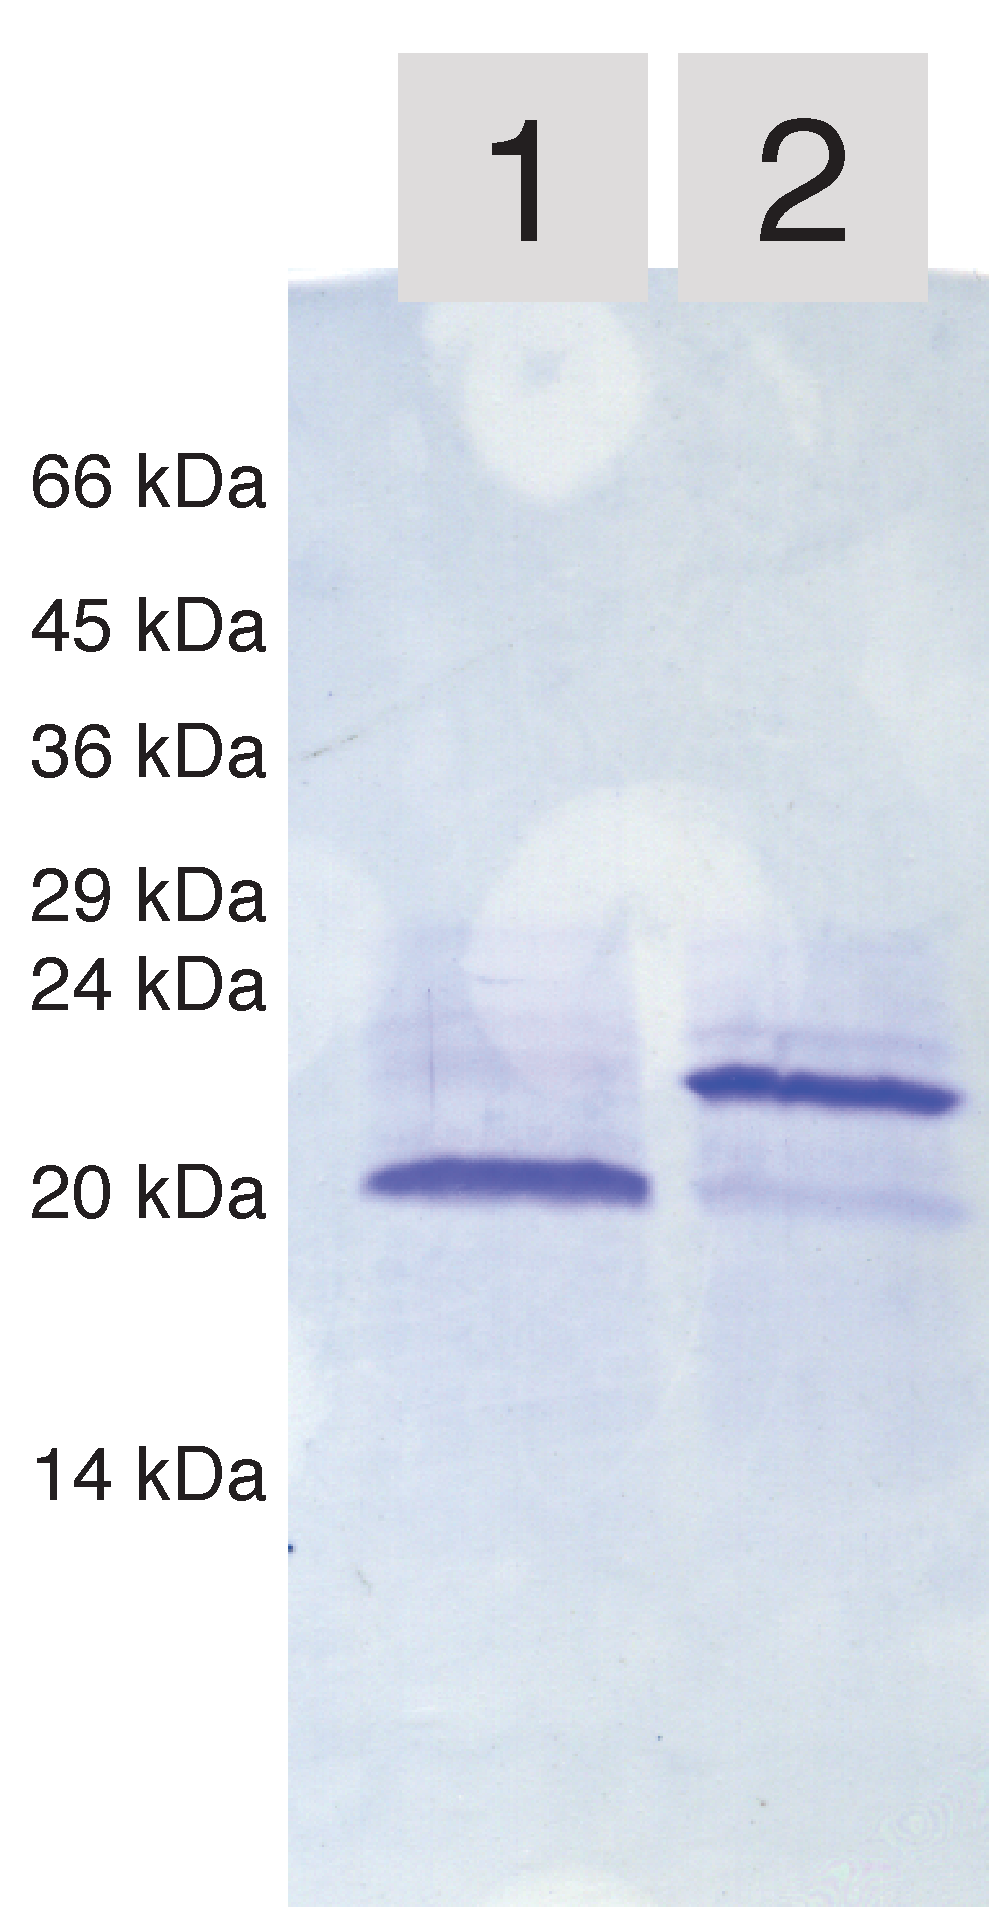
\includegraphics[width=0.2\textwidth]{porin_chapter/img/Fig3-gelpurif.pdf}
   	\end{center}
   	\caption[\ac{SDS-PAGE} showing OmpW from \caulobacter obtained by elution of the 20 kDa band]{
15\% \ac{SDS-PAGE} showing OmpW of \caulobacter obtained by elution of the 20 kDa band from preparative \ac{SDS-PAGE} Lane 1: Molecular mass markers 66 kDa, 45 kDa, 36 kDa, 29 kDa, 24 kDa, 20 kDa, and 14 kDa. Lane 2: 5 \microgram of OmpW solubilized at room temperature for 10 min in 5 \microlitre of sample buffer. Lane 3: 5 \microgram of OmpW solubilized at 100\cel for 10 min in 5 \microlitre of sample buffer. The gel was stained with Coomassie.
   	}
   	\label{fig:porin-elutedband}
\end{figure}   

\subsection{Partial sequencing of the 22 kDa protein of \textit{C. crescentus}}
The 20 kDa protein was subjected to sequencing using Edman-degradation. In a first run the protein could not be sequenced starting from the N-terminus, presumably because of N-terminal blockage. Following trypsin treatment one stretch corresponding to the N-terminal end with a molecular mass of 1764.8 Da could be resolved by sequencing. The sequence of the partial peptide was \texttt{QDFTPNAKGDLIVHAR}, which suggested that the N-terminus was blocked by the formation of pyroglutamate. A \ac{blast} analysis\upcite[]{blast, zhang1997powerblast} of the sequenced peptide unambiguously demonstrated that the 20 kDa protein was OmpW of \caulobacter and was a member of the extensive OmpW-family of outer membrane proteins of Gram-negative bacteria. To ensure that the higher molecular mass band observed in boiled samples was also OmpW; this protein band (about 22 kDa) was also subjected to sequencing following trypsin treatment. Its N-terminal end was identical to that of the 20 kDa protein (OmpW), indicating again that OmpW existed in two different configurations where one was heat-modifiable. 

\subsection{Analysis of the channels formed by OmpW channel-forming protein of \textit{C. crescentus}}

\Cref{fig:porin-20ksinglechannel}B (upper panel) shows a single-channel recording of a \ac{PC} membrane in the presence of the purified OmpW protein of \caulobacter, which was added to a black lipid membrane at a concentration of about 20 \si{\nano\gram\per\milli\litre}. The single-channel recording demonstrates that the protein formed the same defined channels as found in \ac{PBS}-\ac{EDTA} extracted membranes of \caulobacter. The average single-channel conductance was about 125 \si{\pico\sievert} in 1 \si{\molar} \ce{KCl} (almost 40\% of all conductance steps). Only a minor fraction of channels with other conductance was observed (see the histogram in \cref{fig:porin-20ksinglechannel}B, lower panel) suggesting that conductance steps with more than one unit conductance were less frequent for the purified OmpW than for the crude outer membrane fraction. It is noteworthy that the channels formed by OmpW of \caulobacter had a long lifetime, similar to those that have been detected previously for porins of Gram-negative\upcite[]{benz1994uptake} and Gram-positive bacteria\upcite[.]{trias1993characterization, trias1994permeability} All these channel-forming proteins from the cell walls of bacteria form channels in lipid bilayer membranes with long lifetimes at small transmembrane potential (mean lifetime at least 5 min). Furthermore, no voltage-dependence closure was observed in KCl-solution voltages up $\pm$120 mV (data not shown). 

\begin{figure}[p]
  	\begin{center}
   		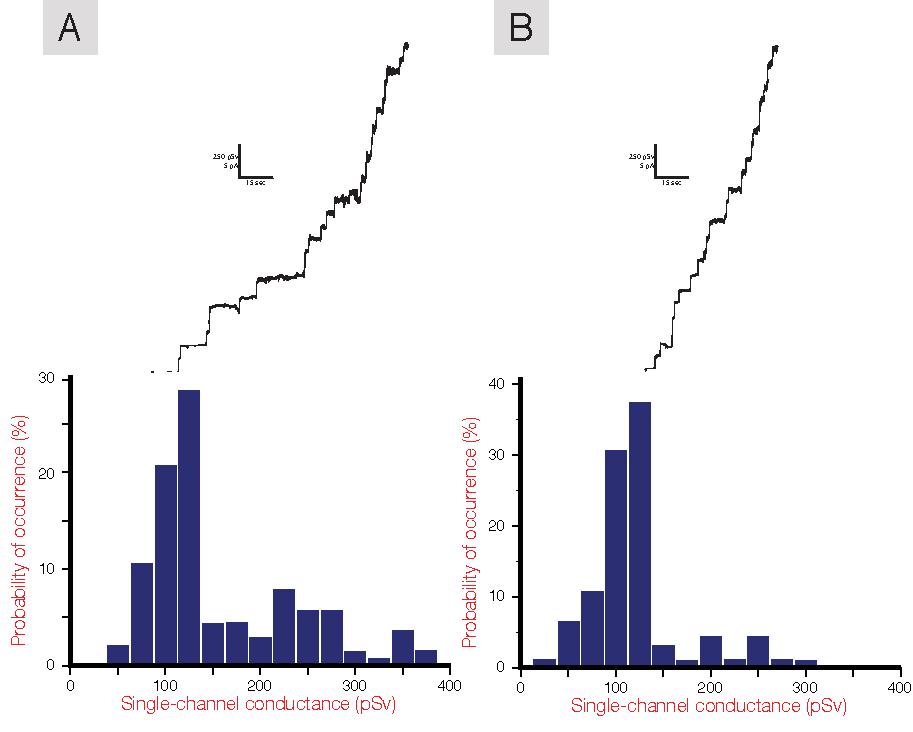
\includegraphics[width=0.8\textwidth{}]{porin_chapter/img/Fig2-singleconductances.pdf}
   	\end{center}
   	\caption[Single-channel measurements with detergent treated outer membrane of C. crescentus and purified 20 kDa protein]{
Single-channel measurements with detergent treated outer membrane of \caulobacter and purified 20 kDa protein.\\
\textbf{A} Upper panel: Single-channel recording of a PC/n-decane membrane in the presence of enriched outer membranes of \caulobacter. The aqueous phase contained 1 M \ce{KCl} and 100 \si{\nano\gram\per\milli\litre} protein from enriched outer membranes treated with 0.5\% \ac{LDAO}. The applied membrane potential was 20 \si{\milli\volt}; T = 20\cel.\\
Lower panel: Histogram of the probability P(G) for the occurrence of a given conductivity unit observed with membranes formed of \ac{PC}/n-decane in the presence of enriched outer membranes of \caulobacter. P(G) is the probability that a given conductance increment G is observed in the single-channel experiments. It was calculated by dividing the number of fluctuations with a given conductance increment by the total number of conductance fluctuations. The aqueous phase contained 1 M \ce{KCl}. The applied membrane potential was 20 \si{\milli\volt}; T = 20\cel. The average single-channel conductance was 125 \si{\pico\sievert} for 105 single-channel events (left-hand maximum). \\
\textbf{B} Upper Panel: Single-channel recordings of a \ac{PC}/n-decane membrane in the presence of purified OmpW of \caulobacter. The aqueous phase contained 1 M \ce{KCl} and 20 \si{\nano\gram\per\milli\litre} OmpW dissolved in 1\% Genapol. The applied membrane potential was 20 \si{\milli\volt}; T = 20\cel. \\
Lower panel: Histogram of the probability P(G) for the occurrence of a given conductivity unit observed with membranes formed of \ac{PC}/n-decane in the presence of OmpW of \caulobacter The applied membrane potential was 20 \si{\milli\volt}; T = 20\cel. The average single-channel conductance was 125 \si{\pico\sievert} for 95 single-channel events.
   	}
   	\label{fig:porin-20ksinglechannel}
\end{figure}   

Single-channel experiments were also performed with salts other than \ce{KCl} to obtain information on the size and selectivity of the channels formed by OmpW of \caulobacter. The results are summarized in \cref{tab:porin-conductance}. The conductance sequence of the different salts within the channel was \ce{KCl} $\approx$ \ce{KOAc} $\approx$ \ce{NH4Cl} \textgreater \ce{RbCl} \textgreater \ce{NaCl} \textgreater \ce{CsCl} \textgreater \ce{LiCl}. The influence of cations of different size and mobility on the conductance was quite substantial (see \cref{tab:porin-conductance}) suggesting indeed high cation-selectivity of the OmpW channel. For more bulky cations such as \ce{N(CH3)4+} or the Tris$^+$ cation we observed a very low conductance of much less than 10 \si{\pico\sievert} suggesting that the size of the OmpW channel is indeed very small. 

\begin{table}[htb]
    \centering
    \caption[Average conductance through OmpW]{Average single-channel conductance of OmpW of \caulobacter in different salt solutions and radii, hydrated radii, and limiting molar conductivity of the cations. This data is also presented in a graphical figure, \cref{fig:porin-ionicradii}}
    \label{tab:porin-conductance}
    \begin{tabular}{@{}lrrrrr@{}}
        \toprule
        Salt      & Concentration & Single-channel  & Ion  & Hydrated Ion  & Limiting Molarity     \\ 
              &  &  conductance &  Radius &  Radius &  Conductivity     \\ 
                  & M             & \si{\pico\sievert}        & nm         & nm                  & \si{\milli\sievert\per\molar} \\ \midrule
        \ce{LiCl}      & 1.0           & 15 $\pm$ 3.0                   & 0.059      & 0.216               & 38.68                           \\
        \ce{NaCl}      & 1.0           & 40 $\pm$ 3.5                   & 0.100      & 0.163               & 50.10                           \\
        \ce{KCl}       & 0.01          & 30 $\pm$ 3.2                   & 0.137      & 0.110               & 73.50                           \\
        --\textquotedbl{}--  & 0.03          & 40 $\pm$ 3.4                   &            &                     &                                 \\
         --\textquotedbl{}-- & 0.1           & 55 $\pm$ 4.9                   &            &                     &                                \\
      --\textquotedbl{}-- & 0.3           & 80 $\pm$ 6.2                   &            &                     &                                 \\
        --\textquotedbl{}--  & 1.0           & 125 $\pm$ 8.1                  &            &                     &                                 \\
        --\textquotedbl{}-- & 3.0           & 150 $\pm$ 8.9                  &            &                     &                                 \\
        \ce{NH4Cl}     & 1.0           & 125 $\pm$ 9.5                  & 0.147      & 0.110               & 73.55                           \\
        \ce{RbCl}      & 1.0           & 100 $\pm$ 7.6                  & 0.152      & 0.105               & 77.81                           \\
        \ce{CsCl}      & 1.0           & 30 $\pm$ 2.9                   & 0.167      & 0.106               & 77.26                           \\
        \ce{N(CH3)4Cl} & 1.0           & \textless10                & 0.347      & 0.182               & 44.92                           \\
        \ce{KAcO-} (pH 7)  & 0.1           & 60 $\pm$ 8.0                   &            &                     &                                 \\
         --\textquotedbl{}-- & 1.0           & 125 $\pm$ 10                   &            &                     &                                 \\
        \ce{CaCl2}     & 0.5           & 225 $\pm$ 22                   &            &                     &                                 \\
         --\textquotedbl{}-- & 1.0           & 250 $\pm$ 19                   &            &                     &                                 \\
        \ce{MgCl2}     & 1.0           & 275 $\pm$ 27                   &            &                     &                                 \\ \bottomrule
    \end{tabular}
\end{table}

An additional significant result of the single-channel measurements was the extreme high conductance of OmpW in \ce{CaCl2} (see \cref{tab:porin-conductance}). In 1 M \ce{CaCl2}, the conductance was about 250 \si{\pico\sievert}; this was again close to saturation because in 0.5 M \ce{CaCl2} the conductance was only little lower than in 1 M solution. Interestingly, conductance traces in \ce{CaCl2} solutions were very noisy suggesting a strong interaction between the divalent cations and the OmpW channels. Similarly, channel-forming activity in salt solutions containing divalent cations was much lower than that in monovalent cation solutions, indicating that OmpW could be a channel for divalent cations, such as \ce{Ca^2+} or \ce{Mg^2+}. \Cref{tab:porin-conductance} also shows the average single-channel conductance, G, as a function of the \ce{KCl} concentration in the aqueous phase. Similarly, as in the case of some channels of Gram-positive bacteria\upcite[,]{trias1993characterization, trias1994permeability, riess1998cell} the conductance was not a linear function of the \ce{KCl}-concentration, which means that OmpW did not form a wide, water-filled channel. The saturation with increasing salt concentration could be caused by point net charges and/or a binding site for ions.

\subsection{The OmpW channel of \textit{C. crescentus} is highly cation-selective}

Additional information about the structure of the channel formed by OmpW of \caulobacter was obtained from zero-current membrane potential measurements in presence of salt gradients. A fivefold \ce{KCl} gradient (100 mM versus 500 mM), across a lipid bilayer membrane in which about 100--1000 OmpW channels were reconstituted, resulted in an asymmetry potential of 35 mV at the more dilute side (mean of 3 measurements). This result indicated preferential movement of \ce{K+} ions over \ce{Cl-} through the channel at neutral pH. The zero-current membrane potentials were analyzed using the Goldman-Hodgkin-Katz equation, see \cref{eq:bhk}\upcite[.]{benz1978formation, benz1985ion} The ratio of the potassium permeability, $P_K$, divided by the chloride permeability, $P_{Cl}$, was about 15 (mean of 3 measurements), indicating high cation selectivity of the channel formed by OmpW (see also Discussion, \cpageref{sec:porin-discussion}). This result was confirmed by measurements with \ce{LiCl} and \ce{KOAc}; we observed under the same conditions as for \ce{KCl}, asymmetry potentials around 32 to 35 mV for fivefold gradients, meaning that Pa/Pc was also in these cases also higher than 10. More precise numbers cannot be expected because small errors of the asymmetry potential result in this range in big variations of the permeability ratio Pa/Pc. Size and mobility of the cations did not influence the cation selectivity of OmpW in contrast to the situation observed previously for general diffusion porins\upcite[.]{benz1985ion}
\begin{equation} \label{eq:bhk}
  E_{m,\text{ion}} = \frac{RT}{F} \ln{ \left( \frac{ P_{\text{ion}}[\text{ion}^{+}]_\mathrm{out}}{ P_{\text{ion}}[\text{ion}^{+}]_\mathrm{in}} \right) }
\end{equation}

\subsection{Knocking out ompW removes channel-forming activity} \label{sec:knocking-out-ompw}

To confirm that the gene product encoded by CCNA\_01475 was indeed responsible for the channel forming activity present in our experiments we removed the genomic copy of the gene with a two-step recombination protocol that is standard in \caulobacter genetics. The resulting strain, \caulobacter \del ompW, was confirmed by \ac{PCR} (data not shown) and \ac{SDS-PAGE}. The \ac{SDS-PAGE} analysis of the knockout compared to wild-type can be seen in \cref{fig:porinknockout}. The band that was identified previously as comprising the channel-forming protein was found to be absent in the ompW knockout. Likewise, the channel-forming activity previously found in our extracts was not present in our ompW knockout extracts. These results support the peptide sequencing in that ompW, CCNA\_01475, encodes for an outer membrane porin.

Interestingly, all attempts scale-down our outer membrane extractions, from large flasks to test tubes, were unsuccessful at producing a sample with a prominent \ac{SDS-PAGE} band near 20 kDa (the OmpW band). It is not clear where the important differences are between a flask-based extraction and a tube-based extraction are. A significant amount of time was spent trying to reproduce our original results, seen in \cref{fig:porin-pbsedtagel}, during the time that the knockout was being constructed; culture volume was not considered a significant variable until very late. The reason for this phenomenon is unknown.

All attempts to determine a phenotype for the knockout strain were inconclusive. We hypothesized that the OmpW was involved with \ce{Ca^2+} uptake and that without OmpW the cells would have reduced fitness under \ce{Ca^2+} limitation. It has previously been shown that \caulobacter does require \ce{Ca^2+} in its growth medium, but that Independence from \ce{Ca^2+} can be achieved and  `calcium-free' mutants' have been isolated\upcite[.]{smit1992s} All recent attempts to produce growth media without \ce{Ca^2+}, in the manner previously published, haven't been successful. It seems that there may be a trace level of calcium contamination of some media components. Nevertheless, no reduction in fitness was observed for our ompW knockout strain compared to wild-type in media replete with \ce{Ca^2+} or in media with significantly reduced \ce{Ca^2+}. In fact, no \textit{in vivo} phenotype of any kind was observed with our strain \caulobacter \del ompW.

\begin{figure}[htb]
  	\begin{center}
   		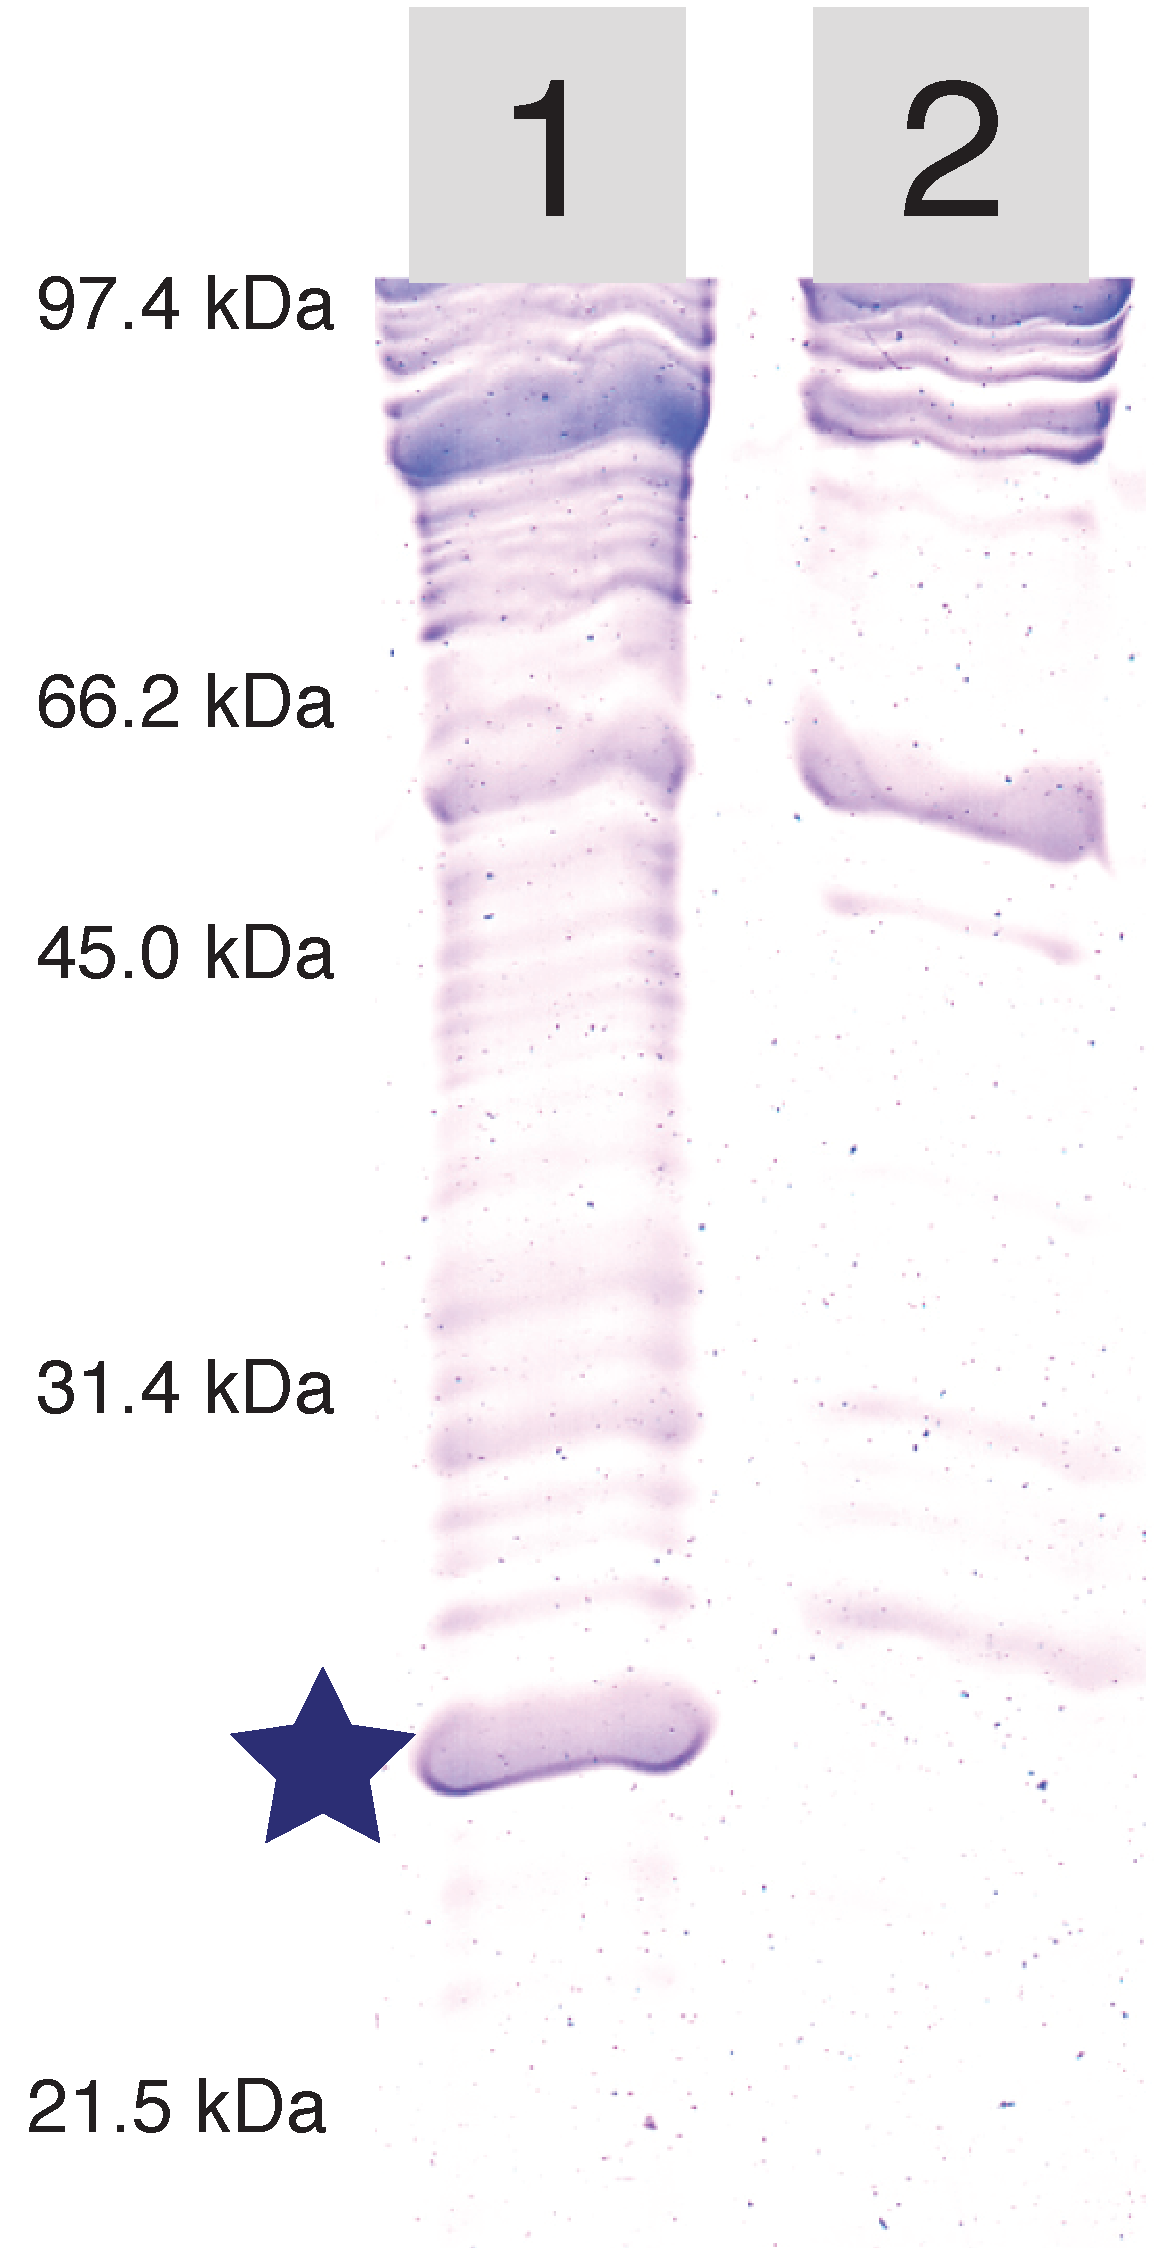
\includegraphics[width=0.2\textwidth]{porin_chapter/img/Fig-knockout.pdf}
   	\end{center}
   	\caption[\ac{SDS-PAGE} of \caulobacter \del ompW]{\ac{SDS-PAGE} analysis of enriched outer membrane preparations of \caulobacter. Lane 1: \caulobacter NA1000. Lane 2: \caulobacter  \del ompW. The star highlights the position of OmpW, the prominent band at 22 kDa. 
   	}
   	\label{fig:porinknockout}
\end{figure}   

\section{Discussion}
\label{sec:porin-discussion}

\subsection{The enriched outer membrane of \caulobacter contains a cation-permeable channel, encoded by ompW}
Here we demonstrated the presence of a channel in the enriched outer membranes of the alpha proteobacterium \caulobacter. Unlike enteric Gram-negatives, the genome does not contain genes that code for the classical outer membrane porins such as OmpC, OmpF, LamB or Tsx\upcite[.]{lohmiller2008tonb, neugebauer2005exbbd, caulobactergenomeseq} Instead the genome of \caulobacter contains 67 genes coding for TonB-dependent receptors\upcite[.]{neugebauer2005exbbd} This suggested that most of the nutrients from the dilute environments where \caulobacter is typically found are actively taken up by TonB-dependent transport systems. Nevertheless, it is clear from this study that \caulobacter also contains an outer membrane channel. The 20 kDa band excised from preparative \ac{SDS-PAGE} had a very high channel-forming activity. No other protein bands excised from gels showed channel-forming activity suggesting that the outer membrane of \caulobacter may contain only one porin-like channel. The channel had a very low single-channel conductance of about 125 \si{\pico\sievert} in 1 M \ce{KCl}. The channel-forming protein was subjected to partial sequencing and was identified as OmpW of \caulobacter. The gene found to encode for the OmpW, CCNA\_01475, was knocked out and the extracts of the resulting strain showed no channel-forming activity.

 The OmpW porin family is widespread amongst Gram-negative bacteria, but with no well established function. Only for OmpW of \ecoli and OprG of \ac{pseudomonas} have channel functions been postulated that may have to do with the uptake of hydrophobic compounds\upcite[.]{hong2006outer, touw2010crystal} In other studies it has been suggested that the channel function of OmpW of \ecoli and OprG of \ac{pseudomonas} may be plugged by W155 and W170, respectively (see \cref{sub:structompw})\upcite[.]{albrecht2006expression, hong2006outer, touw2010crystal} 

Two big-dataset studies out of the Shapiro lab at Stanford University have shed some light on the biology of ompW in \caulobacter; the survey of essential genes by Christen \etal (2011) and the high-throughput analyses of transcription and translation by Schrader \etal (2014). The gene ompW is non-essential for \caulobacter, at least in rich growth medium, \ac{PYE}\upcite[,]{christen2011essential} The gene lies on the forward strand of the genome surrounded by genes of seemingly unrelated function. It is transcribed on to a monocistronic mRNA, while the preceding and succeeding genes are both transcribed on separate polycistronic mRNAs\upcite[.]{schrader2014coding}) The ompW gene is not highly transcribed, nor translated in either rich medium (\ac{PYE})) nor limiting medium (M2G), but interestingly the gene is transcribed at a much higher rate relative rate in rich media than in limiting media while its translation rate remains relatively equal in both media. The differences in transcription rate and translational efficiency between media types was relatively small within to entire study by Schrader \etal, and so it wasn't focused on or discussed in the original study. The reduction in transcriptional activity in minimal medium suggests some transcriptional control, but the translation rate (as measured by ribosome footprinting RNA-seq) remained relatively unchanged (0.9 vs. 0.8 ribosomes per kilobase per million-reads) suggesting that the changes in transcription maybe superseded by a translational control mechanism.

\subsection{Properties of OmpW in the \textit{C. crescentus} outer membrane}
OmpW of \caulobacter was found to be highly cation-selective. Its selectivity for \ce{K+} ions over \ce{Cl-} was at least 10-fold; the calculated value was about 12. However, it has to be kept in mind that the permeability ratio Pa/Pc reacts in this range and is very sensitive to small changes of the asymmetry potential\upcite[.]{benzhancock1987mechanism} This means that we found little indication for the permeation of anions through OmpW because the single channel conductance in 1 M \ce{KCl} was the same as in 1 M \ce{KOAc}, despite the fact that chloride in the aqueous phase has a much higher mobility than acetate. In addition, the single channel conductance was not a linear function of the bulk aqueous salt concentration, see \cref{tab:porin-conductance}. Instead the conductance showed strong saturation; at 3 M \ce{KCl} conductance was only slightly higher (150 \si{\pico\sievert}) than at 1 M \ce{KCl} (125 \si{\pico\sievert}). Similarly, at 0.3 M \ce{KCl}, conductance was only little smaller (80 \si{\pico\sievert}) than at 1 M \ce{KCl}. Experiments with different alkaline cations indicated clearly that OmpW does not form an aqueous pore, which would be typical for most Gram-negative and Gram-positive bacterial porins, even if they contained point charges\upcite[.]{benz1994uptake, riess2000discovery} Instead OmpW of \caulobacter appeared to be an ion channel; its single channel conductance had a maximum for ammonium and potassium ions and became much smaller for bigger cations indicating that they likely loose part of their hydration shell while moving through the channel. This argues for a small selectivity filter inside the channel. Presumably, the ionic radii of the different cations and not the sizes of their hydration shells, play an important role for their permeation through OmpW as \cref{tab:porin-conductance} clearly indicates. \Cref{fig:porin-ionicradii} shows the single channel conductance of OmpW as a function of the ionic radii of the ions\upcite[.]{pauling1960nature, shannon1976revised, smirnov1997ammonium} The conductance data for another small substrate-specific channel (LamB of \ecoli) is given for comparison\upcite[.]{benz1987mechanism} The relationship for OmpW follows approximately the Eisenman series VI for carrier-mediated transport of cations or for the transport of monovalent cations through channels\upcite[.]{eisenman1983ionic} This means presumably that the field strength inside the channel is presumably medium-sized. Ion transport trough general diffusion channels of enteric bacteria follow instead Eisenman series I or II indicating low field strength in the channels. The minimum diameter of OmpW is presumably close to that of \ce{Cs+} or smaller than that of \ce{N(CH3)4+} ions because larger organic cations have a very low permeability through OmpW, if any. 

\begin{figure}[htb]
  	\begin{center}
   		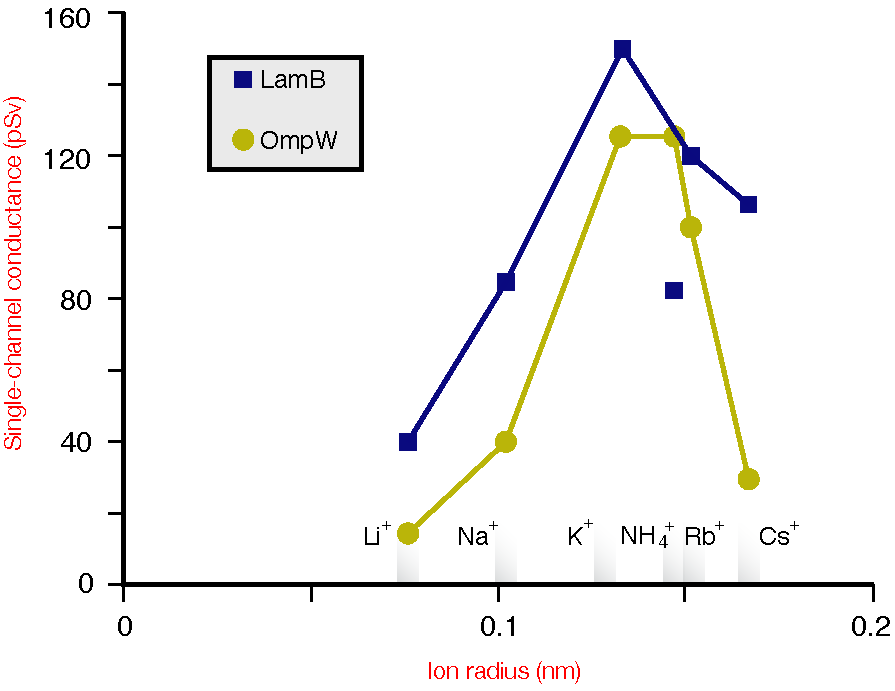
\includegraphics[]{porin_chapter/img/Fig4-conductancegraph.pdf}
   	\end{center}
   	\caption[Single-channel conductance of OmpW in 1 M salt solution as a function of the ionic radii of monovalent cations]{
Single-channel conductance of OmpW in 1 M salt solution as a function of the ionic radii of monovalent cations. 
The data were taken from \cref{tab:porin-conductance}. The single-channel conductance through LamB of \ecoli is given for comparison (data taken from \fullcite{benz1986pore}).
   	}
   	\label{fig:porin-ionicradii}
\end{figure}   

OmpW of \caulobacter clearly functions as a cation-permeable channel, having a preference for divalent cations, since calcium and magnesium ions had a higher permeability through OmpW than potassium ions. This could indeed mean that it is a channel for the transport of calcium and/or magnesium ions. It is extraordinary that such a function has not previously been established for OmpW. The reason for this is that OmpW is a rather small channel with only eight beta strands and so has little possibility for the passage of solutes. Previous data from structural studies of OmpW of \ecoli and OprG of \ac{pseudomonas} suggested that members of the OmpW family could be involved in the transport of small hydrophobic molecules across the bacterial outer membrane\upcite[.]{hong2006outer, touw2010crystal} It is also possible that they are blocked\upcite[.]{albrecht2006expression} Lipid bilayer experiments with OmpW of \ecoli suggested that it forms small ion-permeable channels with a conductance of about 20 \si{\pico\sievert} in 1 M \ce{KCl}\upcite[,]{hong2006outer} which is considerably lower than that of \caulobacter OmpW. The 3-D structure of \ac{pseudomonas} OprG, another member of the OmpW family, was resolved at 2.4 \AA resolution\upcite[.]{touw2010crystal} Again the structure suggested that OprG forms a channel for the diffusion of small hydrophobic molecules, although lipid bilayer experiments proposed a single-channel conductance of about 500 \si{\pico\sievert} for OprG\upcite[.]{mcphee2009major} This means that OmpW of \caulobacter forms a channel that has, despite sequence homologies with OmpW of \ecoli and OprG of \ac{pseudomonas} (see below), a completely different function than other outer membrane proteins.

\subsection{Structure of OmpW of \textit{C. crescentus}}\label{sub:structompw}
Sequence comparison, \ac{blast}, of OmpW of \caulobacter with other members of the OmpW family suggested that it had highest homology with OmpW of \textit{Caulobacter segnis} ATCC 21756, \textit{Asticcacaulis excentricus} CB 48, \textit{Brevundimonas} sp. BAL3, and \textit{Phenylobacterium zucineum} HLK1\upcite[.]{blast, zhang1997powerblast} These bacteria are closely related to the genus \textit{Caulobacter}, belonging to the family \textit{Caulobacteraceae}, order \textit{Caulobacterales}. All these OmpW polypeptides are similar in length to \caulobacter OmpW (200--250 amino acids) and share many strategically positioned conserved residues. The homology of the \caulobacter OmpW to the OmpW proteins with known 3D structure (OmpW of \ecoli and OprG of \ac{pseudomonas}) is less pronounced, but still obvious (amino acid identity is approximately 32\% in both cases and and 19.4\% for all three proteins  (Hong et al., 2006; Touw et al., 2010). 41 amino acids, including many glycines and several prolines, appear to be highly conserved between all three OmpW family proteins. This allows a meaningful comparison between the three different OmpW species (see \cref{fig:porin-seqalign}) and it is also possible to built the possible structural model of OmpW of \caulobacter using homology modeling approach\upcite[]{eswar2008protein} (see below). 

\begin{figure}[htb]
  	\begin{center}
   		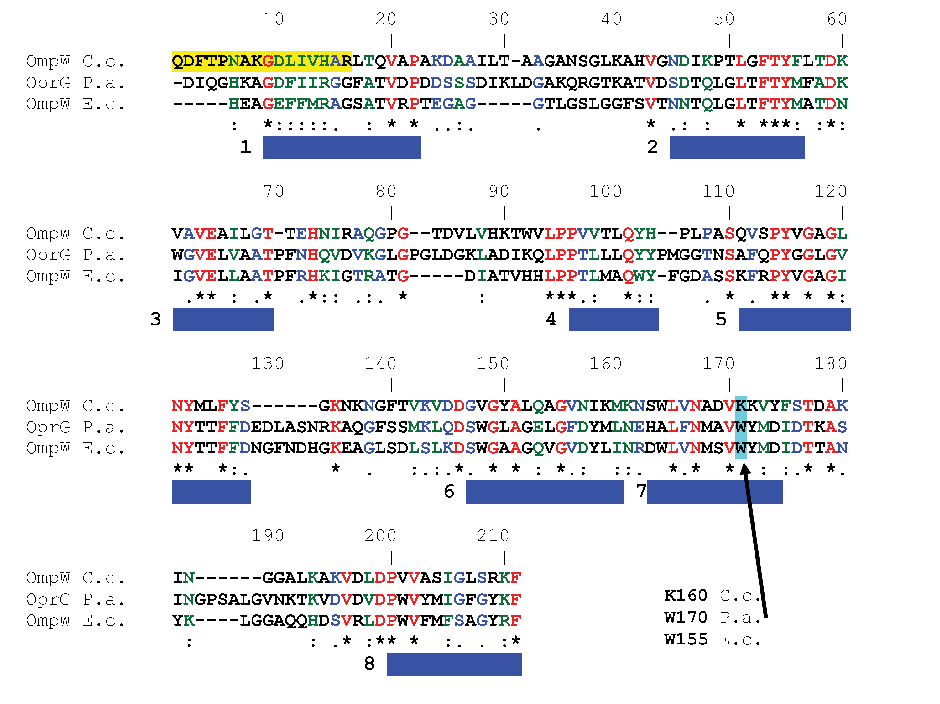
\includegraphics[]{porin_chapter/img/Fig5-seqalign.pdf}
   	\end{center}
   	\caption[Amino acid sequence alignment of OprG of \ac{pseudomonas}, OmpW of \ecoli, and OmpW of \caulobacter]{Amino acid sequence alignment of OprG of \ac{pseudomonas}, OmpW of \ecoli, and OmpW of \caulobacter.
The alignment was performed using Pole Bioinformatique Lyonnaise Network Protein Sequence Analysis (\url{http://npsa-pbil.ibcp.fr}). Amino acids identical in all three proteins are highlighted in red, strongly similar amino acids (:) are given in green and weakly similar ones (.) in blue. The replacement of W155 of OmpW of \ecoli and W170 of OprG of \ac{pseudomonas} by K160 of \caulobacter is given in green color and is indicated by an arrow. The eight beta strands in OprG of \ac{pseudomonas} and in OmpW of \ecoli are numbered and indicated by blue bars. The yellow highlighted sequence was found by N-terminal sequencing of OmpW of \caulobacter.
   	}
   	\label{fig:porin-seqalign}
\end{figure}   

Crystal structures of \ecoli OmpW\upcite[]{hong2006outer} and \ac{pseudomonas} OprG\upcite[]{touw2010crystal} suggested the formation of hydrophobic channels for these proteins and they are believed to be responsible for the passage of hydrophobic solutes across the bacterial outer membrane. Small and hydrophobic \ecoli OmpW channel has a conductance of approximately 20 \si{\pico\sievert} in 1 M \ce{KCl}\upcite[.]{hong2006outer} In contrast, the \caulobacter OmpW formed a channel with a relatively high conductance of 125 \si{\pico\sievert} in 1 M \ce{KCl} in our bilayer measurements. A comparison of the structures of these OmpW family proteins revealed factors that might lead to a larger conductance in \caulobacter OmpW. Crystal structures suggested that both \ecoli OmpW and \ac{pseudomonas} OprG form a hydrophobic gate (\cref{fig:porin-models}A; b and c) in the central region of the channel. Both channels have an aromatic, bulky and hydrophobic tryptophan residue as a part of a hydrophobic gate, which may make the passage of ions through channels difficult. Similarly, W155 of OmpW of \ecoli\upcite{hong2006outer} and W170 of OprG of \ac{pseudomonas}\upcite[,]{touw2010crystal} which are both considered as plugs of the channels are replaced in OmpW of \caulobacter by K160. This may indicate that this channel has a function different from that of the homologs in \ecoli and \ac{pseudomonas} In addition, \caulobacter OmpW has a hydrophilic and relatively less bulky lysine residue at the corresponding position (\cref{fig:porin-models}A; a), which is unlikely to hinder passage of ions through the channel. In addition, the \caulobacter OmpW has a relatively more hydrophilic interior environment of the channel (\cref{fig:porin-models}A; a), as shown by green color surface within the black box) as compared to the \ecoli OmpW (\cref{fig:porin-models}; b) and the  \ac{pseudomonas} OprG (\cref{fig:porin-models}; c). For \ecoli OmpW and \ac{pseudomonas} OprG the interior surface of the channel is hydrophobic (white color surface), which could make the permeation of ions through the channel energetically unfavorable. \caulobacter OmpW, on the other hand, due to its relative hydrophilic environment may not provide the permeation barrier to ion passage, resulting in a relatively higher conductance of the channel. 

\begin{figure}[htb]
  	\begin{center}
   		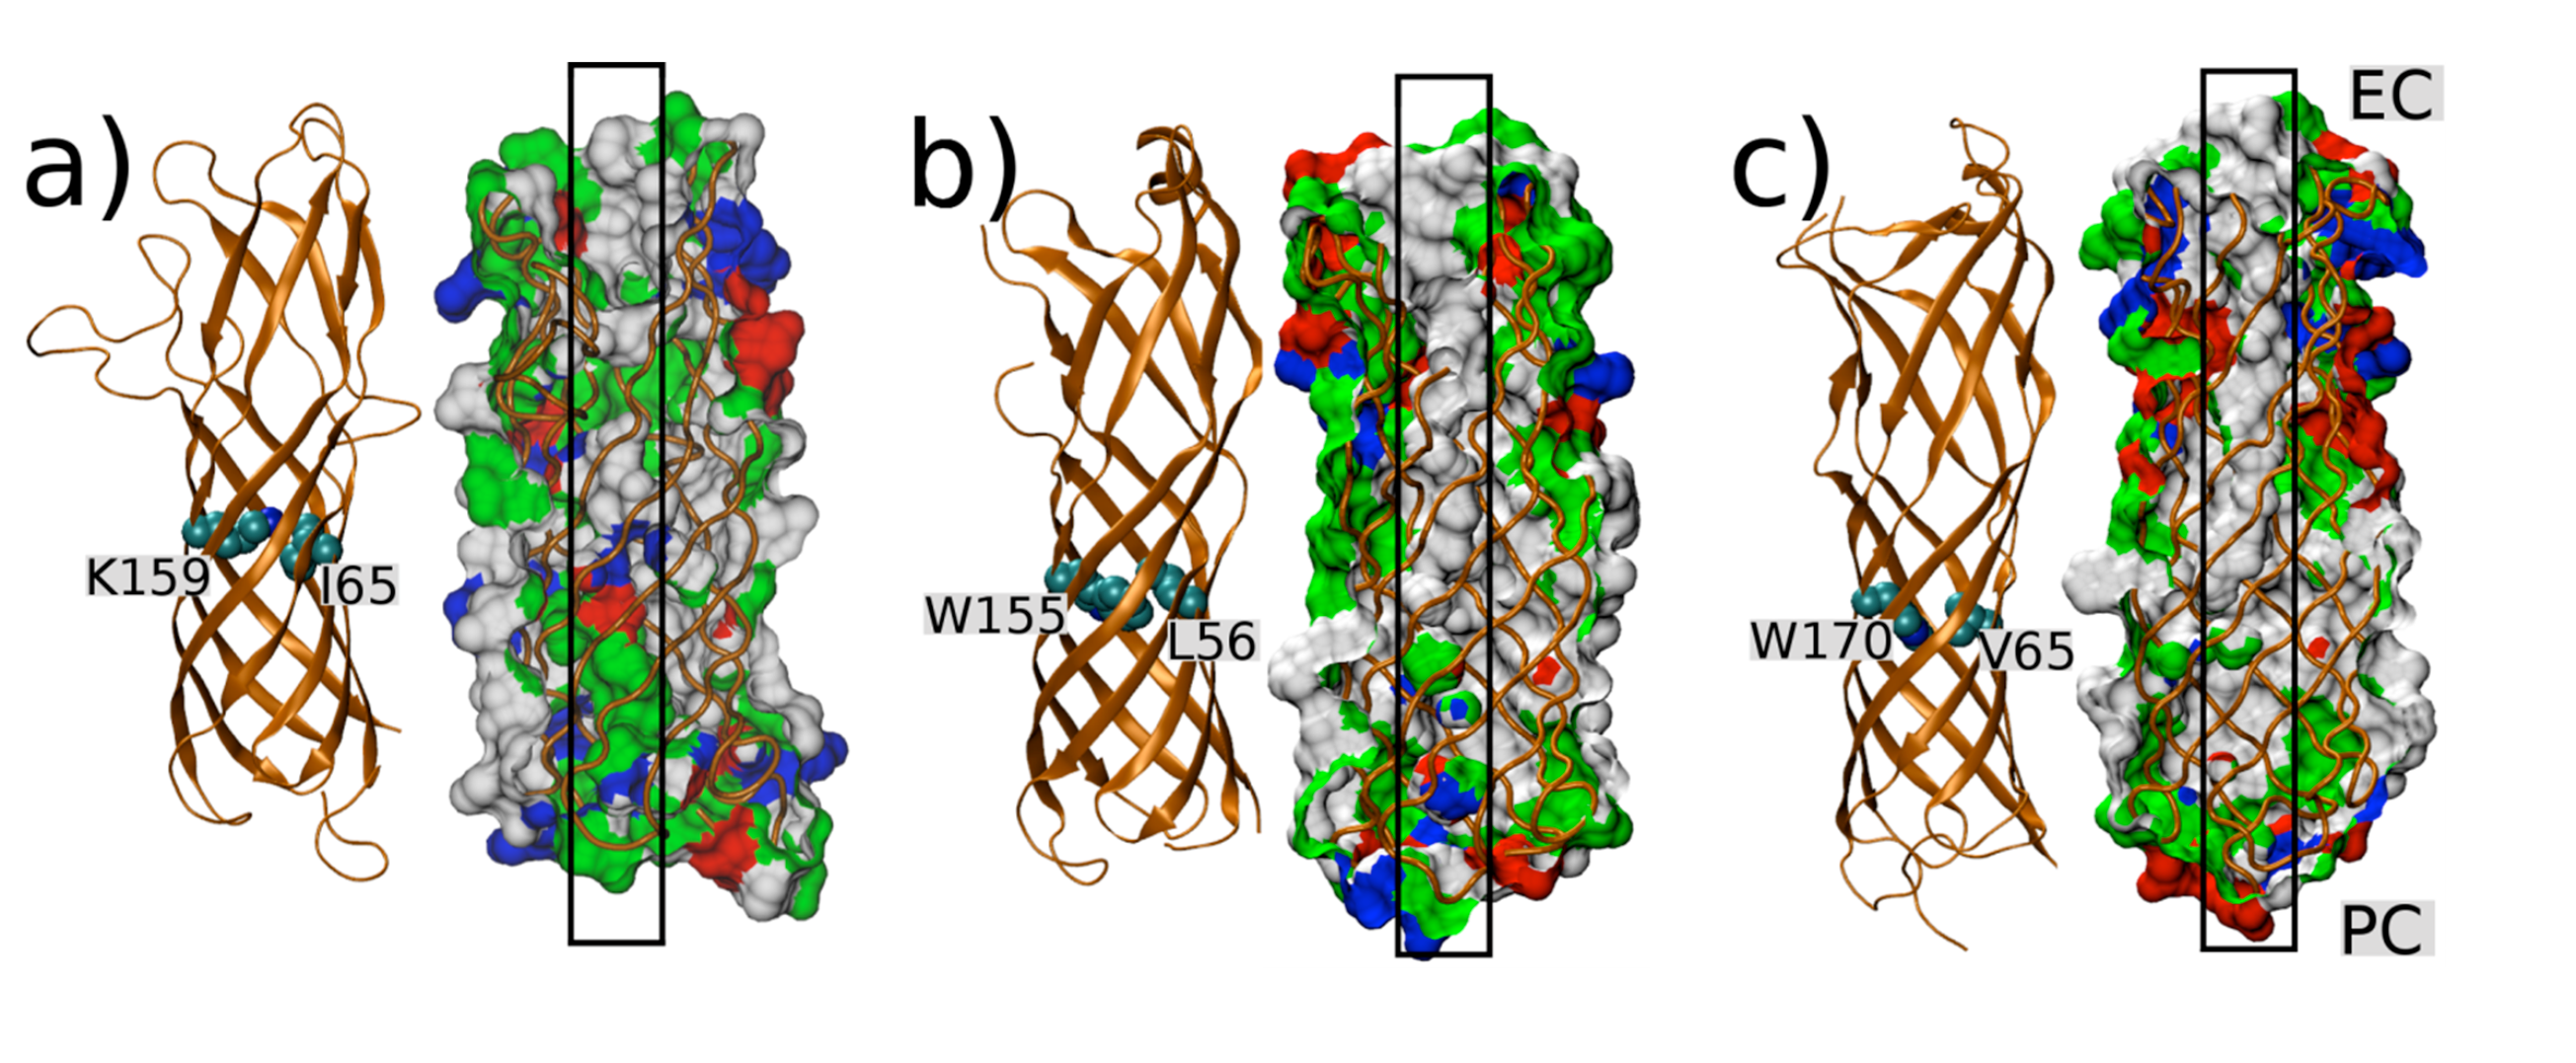
\includegraphics[width=\textwidth]{porin_chapter/img/Fig6a-models.pdf}
   	\end{center}
   	\caption[Structural properties of OmpW of \caulobacter]{
      Comparison of structural features between a) OmpW \caulobacter b) OmpW \ecoli c) OprG \ac{pseudomonas}. Residues, which are a part of a putative hydrophobic gate in \ecoli (W155 and L56) and \ac{pseudomonas} (W170 and V65) channels are shown as spheres. Corresponding residues in OmpW \caulobacter (K159 and I65) are also shown. Additionally all the channels are shown as a surface representation and color coded according to residue type (Green: hydrophilic, white: hydrophobic, red: acidic, blue: basic). Channels are cut from the front to enable visualization of interior channel surface. Black colored box indicate a putative ion transport pathway across the channel. EC and PC denote extracellular and periplasmic sides of the channel respectively.
   	}
   	\label{fig:porin-models}
\end{figure}   

\begin{figure}[htb]
  	\begin{center}
   		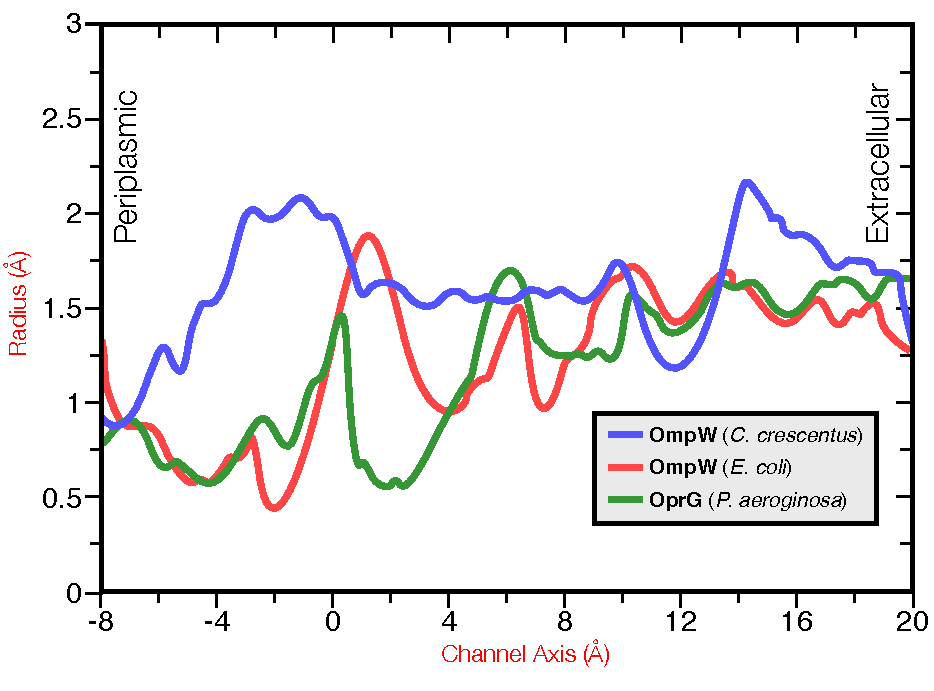
\includegraphics[]{porin_chapter/img/Fig6-poresizes.pdf}
   	\end{center}
   	\caption[Comparison of porin channel radii]{
Comparison of channel radii between \caulobacter OmpW (blue), \ecoli OmpW (red) and OprG of \ac{pseudomonas} (green) along the channel axis. The channel radii were calculated using the program \texttt{HOLE} (\fullcite{smart1996hole}). The extracelluar side is indicted along the right side and the periplasmic side is indicated along the left side.
   	}
   	\label{fig:porin-poresizes}
\end{figure}   

We also examined the contribution of the size of the pore towards higher conductance of \caulobacter OmpW. We observed a slightly larger radius of \caulobacter OmpW channel as compared to other two channels in several regions, particularly from the center of the channel towards the periplasmic side (\cref{fig:porin-poresizes}). Another important feature of the OmpW family channels from \ecoli and \ac{pseudomonas} is the presence of a lateral opening in the barrel wall, which is suggested to allow diffusion of small hydrophobic solutes across the outer membrane by a lateral diffusion mechanism\upcite[.]{hong2006outer, touw2010crystal} In our modeled structure of \caulobacter OmpW, we do not observe such an opening in the channel which further supports the view that the \caulobacter channel may have a different function from that of \ecoli OmpW and \ac{pseudomonas} OprG. Interestingly, the structure of OprG shows additional short beta-strands (not shown in \cref{fig:porin-seqalign}) that are not membrane spanning. These beta-strands seem to extend over the thickness of the outer membrane, which means that they form long external loops\upcite[.]{hong2006outer, touw2010crystal} The solved structures OmpW from \ecoli and OprG from \ac{pseudomonas} provide examples of  successful crystallization efforts for this class of protein and they are exciting starting points for future work towards improving the structural knowledge of OmpW from \caulobacter.

\caulobacter has a requirement for calcium, though it is not clear where the absolute requirement lies. \ce{Ca^2+} ions are needed for assembly of the crystalline \ac{S-layer} RsaA\upcite[.]{nomellini1997factors}. Since RsaA is secreted by a type I secretion mechanism, it is likely that calcium is also needed for either secretion or folding of the protein following secretion, in a manner analogous to all other type I secreted proteins.  However, the \ac{S-layer} a completely dispensable structure. Moreover, the type 1 secretion apparatus spans both the cytoplasmic and outer membranes; hence for \ac{S-layer} there is no apparent need for a channel that enables \ce{Ca^2+} ion movement to the periplasm. There are, however, additional still undefined roles for \ce{Ca^2+} ions. Mutants no longer requiring calcium compounds for growth can be isolated\upcite[.]{walker94} One consequence of all these mutants is the loss of the \ac{OPS} of \ac{LPS} that is used for \ac{S-layer} attachment. As a consequence, these so called `calcium-independent' mutants all shed RsaA into the culture medium. This causal relationship has not been deciphered, but since \ac{OPS} biosynthesis involves synthesis activities within the periplasmic space, it may be that a calcium selective OmpW porin plays a specific role in this process. Here we have provided clear evidence that OmpW could be responsible for the uptake of cations, especially divalent cations, like \ce{Ca^2+} in \caulobacter. 
